\documentclass{article}
\usepackage[utf8]{inputenc}

\usepackage[english]{babel}
\usepackage{subfig}
\usepackage{graphics}
\usepackage[export]{adjustbox}
\usepackage{fancyhdr}
\usepackage[export]{adjustbox}
\usepackage{csquotes}

\usepackage{biblatex}
\addbibresource{references.bib}

\usepackage{hyperref}
\hypersetup{
    colorlinks=true,
    linkcolor=blue,
    filecolor=magenta,
    urlcolor=blue,
}
\setlength{\parskip}{1em}
\title{Sustainable programming through good and clean code.\newline
    DA115A Methods for Sustainable Programming Report,7.5 credits,
    for the degree of Bachelor of Science in software development
    Autumn Semester 2020 Faculty of Natural Science.}
    
\author{(Osagie Osahenagharu (osahenagharu.osagie0005@stud.hkr.se)}

\date{February 19 2021}

\begin{document}

\tableofcontents

\maketitle

\pagestyle{fancy}
\rfoot{
\includegraphics[width=5cm,right]{report_Images/Picture 1.png}}
\setlength{\footheight{35.10004pt}
\setlength{\footskip}{109.98813pt}
\newpage 
\section{Abstract}
Learning programming is hard and strenuous. but the key is persistence.
Through my short period as a "programmer in the making", I have come to realize
that to be successful in this branch of Information technology, one must be a thinker, 
creative, and follow strict rules and guidelines in other to maintain relevance and
sustain pro efficiency. Studying the module, Method for sustainable programming is a
good insight into the standard and requirement of the industry and now to a degree,
one can say that I am better equipped with the need and requirements of the industry.
This report talks about challenges, methods, and tools employed to achieving sustainable programming 
with good and clean code in focus.
\newpage 
\section{Background}
Maintaining a long-living software system is substantially related to the quality of the code the system is built from. This report analyses how good and clean code makes programming sustainable and its usefulness on the early stage of my examination 2 project. The Tools and practices have been used with an immediate effect of having cleaner code that is easier to understand in the long term. Additional attention is given to the cultural aspect that is involved in reaching a mindset that will allow to set and uphold code quality standards. Reaching a common understanding is a team effort that requires "leaving one's comfort zone". Finding common ground can significantly decide about failure or success in creating maintainable code.
\newpage 
\section{Introduction}
\begin{quote}
    "Any fool can write code that a computer can understand.Good programmers write code that humans can understand."\cite{jayaraman_planning_nodate}
\end{quote}


Although programming has been a hot topic in education for decades, students  still tend to disregard the meaning of good working habits and programming practises. While sustainable programming has proved effective in terms of maintaining code products and optimisation, the process to achieving sustainable programming through good and clean code can be brutal especially for newbies and intermediate programmers who are forced to raised their game due to the high learning pace of the current course being studied.In a recent project conducted by me and my classmates,OP(object oriented)  was combined with functional programming which means that the output produced by a function should not change for a given set of inputs helped a great deal to help me write cleaner and good code, thus helping me to focus on what should be done rather than how  it is done. A new layer of thinking and organisation was birthed as a result of this.Other tools 
was required for this small project aforementioned above in other to achieve our common goal which in the bigger picture represent Sustainable programming and practises.They include TDD,Programmers  development environment,common practises and approach,documentation all of which we would look into in context below.

\newpage
\section{Methods}

Observations from the group work in assignment 02
I really did like the group work.Taking into contest the benefits or just plainly viewing the whole project from an individualistic stand point of view,I would like to say that the mindset and engagement was alike and inspiration was not far fetched as we were pretty much on the same skill level when it comes to our coding skills. A careful look at behavioural changes and problem solving, it turns out that with proper planning(we had a couple of meetings during the cause of the project) has geared us towards the right direction, maintained the connection and harmony to actually understanding the task at hand and even collectively  realising how TDD has helped and improved us in the way we see coding today.

Studies of the outcome of A02, the actual code base


The evidently use of a repository for this project was very insightful and change the overall view of the so many changes that takes place despite actually sharing monolithic code-base between me and my team. I really love the idea of working together as a team and despite not being satisfied by the outcome,it turns out that the actual codebase was easy to manage and new tools was added to our coding memory bank.

Literature studies on unit testing, TDD and good code
nit testing is an essential instrument in the toolbox of any serious software developer. However, it can sometimes be quite difficult to write a good unit test for a particular piece of code. Having difficulty testing their own or someone else’s code, developers often think that their struggles are caused by a lack of some fundamental testing knowledge or secret unit testing techniques.But we might ask,How is unit testing related to good code?
Well literally testing your code means you can guarantee your team and customers that the product is safe and a "sort" of leverage is placed when one unit test every part of a product before its delivered. A quick research done by Alfred Melons shows that programmers who test their code proved more effective than those who did not.Bottom line it feels good to know that whatever code we deliver is safe and can be easily fixed if it has been rigorously test prior to delivery.Essentially, a unit test is a method that instantiates a small portion of our application and verifies its behavior independently from other parts. A typical unit test contains 3 phases: First, it initializes a small piece of an application it wants to test (also known as the system under test, or SUT), then it applies some stimulus to the system under test (usually by calling a method on it), and finally, it observes the resulting behavior. If the observed behavior is consistent with the expectations, the unit test passes, otherwise, it fails, indicating that there is a problem somewhere in the system under test. These three unit test phases are also known as Arrange, Act and Assert, or simply AAA.\cite{Sergey_unit_2017}

A unit test can verify different behavioral aspects of the system under test, but most likely it will fall into one of the following two categories: state-based or interaction-based. Verifying that the system under test produces correct results, or that its resulting state is correct, is called state-based unit testing, while verifying that it properly invokes certain methods is called interaction-based unit testing.

As a metaphor for proper software unit testing, imagine a mad scientist who wants to build some supernatural chimera, with frog legs, octopus tentacles, bird wings, and a dog’s head. (This metaphor is pretty close to what programmers actually do at work). How would that scientist make sure that every part (or unit) he picked actually works? Well, he can take, let’s say, a single frog’s leg, apply an electrical stimulus to it, and check for proper muscle contraction. What he is doing is essentially the same Arrange-Act-Assert steps of the unit test; the only difference is that, in this case, unit refers to a physical object, not to an abstract object we build our programs from.

Another approach to achieving good and maintainable programming is the use of static code analysis to show the code measure and overall quality of the code.Below is the comparison with one of the group which i happen to review the  project.This report would be shallow without actually showing raw data from the actual promise, so if you are actually interested in the analysing of the project metric wise, it is my honor to serve you some statistics about the code project.

Measure the code size
\begin{figure}[h!]
  \centering
  \subfloat[My group Project]{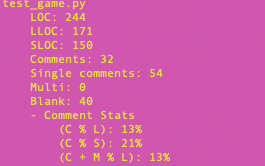
\includegraphics[width=0.4\textwidth]{report_Images/Raw_code_metrics_test game .png}\label{fig:f1}}
  \hfill
  \subfloat[Group B]{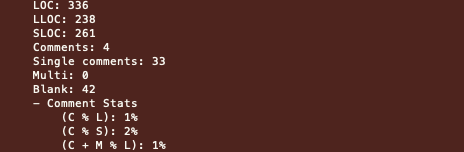
\includegraphics[width=0.4\textwidth]{report_Images/Raw_code_Metrics_test game Group B.png}\label{fig:f2}}
  \caption{Measuring code size}
\end{figure}


Measure the number of test objects, test cases and code coverage
\begin{figure}[h!]
  \centering
  \subfloat[Flower one.]{\includegraphics[width=0.4\textwidth]{flower1.jpg}\label{fig:f1}}
  \hfill
  \subfloat[Flower two.]{\includegraphics[width=0.4\textwidth]{flower2.jpg}\label{fig:f2}}
  \caption{My flowers.}
\end{figure}

Measure the number linter errors
\begin{figure}[!h]
  \centering
  \subfloat[Group B project.]{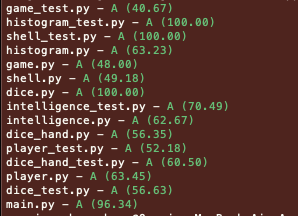
\includegraphics[width=0.4\textwidth]{report_Images/Maintainability Index(visual studio version).png}\label{fig:f1}}
  \hfill
  \subfloat[My project.]{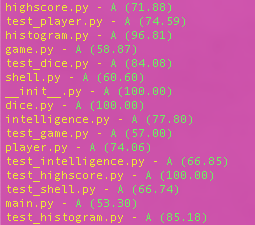
\includegraphics[width=0.4\textwidth]{report_Images/maintability_visible_index.png}\label{fig:f2}}
  \caption{My flowers.}
\end{figure}

Measure quality metrics using static code analysis
\begin{figure}[h!]
  \centering
  \subfloat[group B project.]{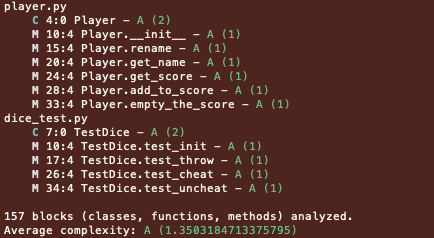
\includegraphics[width=0.4\textwidth]{report_Images/cyclomatic complexity.png}\label{group B project}}
  \hfill
  \subfloat[My project.]{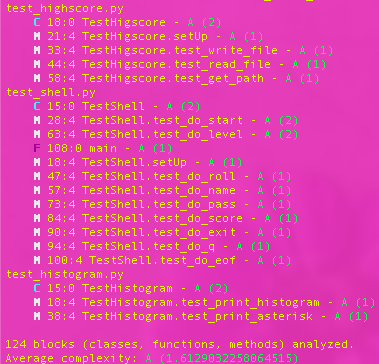
\includegraphics[width=0.4\textwidth]{report_Images/cyclomatic_complexity_our project.png}\label{images}}
  \caption{Cyclomatic complexity in focus}
\end{figure}

\newpage
\section{Results}

I started my IT journey at HKR having taking programming 1 online early last year and my approach has always been the same.i always put more effort into writing code or implementing required functionality or even thinking of how to solve the problem directly without really taking a step back and doing proper analysis. I tried to write code as per my best, but most of the time I faced difficult times during coding sessions.Through the development of this course,I have increased working hours and struggling to fix the never ending bugs be it in modifying an existing application or writing a product or project from base.This was also experienced by the whole team in the just concluded examination 2 of this course. The whole team was spending day and night, including weekends, and output was not so satisfactory if i must admit,because this process is fairly new and its a lot to absorb.  During the time working as a team member I was thinking it was as a result of bad estimates and poor planning because the code was written before the unit test,because me and my team struggled to see how we could write the test for the functionality of the project before the actual project.It was a real challenge to get these rules followed by the entire team,as we have never written any or done any proper unit test for our codes previously.One strong point made by the team was how can one write a test case without implementing the functionality. I myself had the same question initially, but it was misguided. Writing test cases prior to development, led us to think about the functionality as per the end  output. Eventually all of us agreed it made good sense to write tests first. Moving forward we reviewed our progress after couple of releases to find out if it was really helpful and whether it made sense to continue to do so But after the projected was completed, i could reflect and start to see why it was super important to write test for the project before the actual code  as .In order to follow the organization’s standard and best practices,we decided to focus more on the TDD aspect where we  wrote the test cases along with Pass/Fail status. It was really a very good practice since it ensures that particular functionality has been well tested .And  now,i have developed my own guidelines for meaningful project henceforth which are,
Writing first the unit test cases in document related to any functionality prior to writing the code.Then i would track changes to the document.make the status of that test case as fail, since no code has been written to implement that functionality.Writing just enough code to implement the functionality, run the unit test cases written for that functionality and update the status,track changes to ensure that test cases has been written first and tested later.We had some findings after our last release.
We got a better understanding of functionality and able to visualize the behavior more appropriately.We were able to discover additional possible test scenarios including positive and negative tests and accordingly implement in the code.
We  got more confidence with our implementation, because of the greater test coverage.

The remaining challenge was regression testing and the re-testing of previously written code because of responding to change. This would have been impractical with our manual process because of how long it would take. hopefully releases in the future with team mates would be much more stable.TDD makes development more predictable, allowing for more accurate time
estimations and less stress on the developers [2, 3, 23]. It allows developers
to make changes to code without the fear of it breaking. It alleviates the
risk of small changes and refactoring. Large changes are equally risk-free
when broken up into smaller ones as suggested in [24]. By following the
aforementioned three-rule loop and by adhering to small incremental changes,
manual testing and debugging become unnecessary as broken tests indicate
broken code added in the previous loop.TDD encourages good design by enforcing decoupling, leading to easily testable code

\newpage 

\section{Analysis and Discussion}
\subsection{ unit testing}
   Unit testing is a fundamental practice in Extreme Programming but most nontrivial code is difficult to test in isolation. You need to make sure that you test one feature at a
time, and you want to be notified as soon as any problem occurs. Normal unit testing is hard
because you are trying to test the code from outside.
    Beck popularized the concept of test-driven development (TDD) in\cite{kong_chapter_2021}, presenting a loop of “red, green, repeat” — red and green meaning failing and
passing tests, respectively. Martin describes the system further as a
loop consisting of three rules. First, before writing production code, there
needs to be a failing unit test. Second, that unit test must not be any longer
than is needed for it to fail. Third, enough production code must be written
to make the test succeed and no more. According to Martin, this loop should
ideally last only a few minutes.Tightly coupled functions are difficult to test. Ideally, the tests are minimal and test only one function, but they cannot if that function calls other functions or has side effects.Refactoring is the process in which the code’s structure is improved by rewriting and restructuring it without changing its behavior notes that while traditionally software has been meticulously designed beforehand in order to avoid having to rewrite any of it, in modern programming.

\newpage 
\subsection{documenting software.}
     Good tests act as documentation for the rest of the code base. They should thus be treated like any other code.readable, simple and clean.
    \newpage 
    
\subsection{good and clean code, try to explain what it is and how should one proceed in learning how to write good and clean code}
\newpage 

\subsection{importance of the programmers development environment and how important it might be, or not, for the programmers productivity in delivering good and clean code.}
\newpage 

\subsection{Use software philosophies/principles (learnt from lecture) and relate those to your group work for A02. What principles did you use and what principles do you think you should have discussed to use in the project?}
\newpage 
    
\subsection{Elaborate and write on the topic "sustainable software development", in your own view, what are the essentials?}
\newpage 

\subsection{Use static code analysis tools to measure your own project and the one you opposed on. Gather the metrics into the report and elaborate on how well the data is showing properties of good and clean code}

\newpage 
\section{Summary}
My development journey continues. But what I have learned and found very appealing about agile development is it includes testing and coding concurrently. This is exactly what TDD emphasizes through its mantra. The transformation, from coder to developer, is needed in all agile software development projects.
Write a final section of your report where you summarize your findings and hit about future work and where to go from here.



\newpage 

\printbibliography

\end{document}
